%
% 2-fundamtenallemma.tex
%
% (c) 2023 Prof Dr Andreas Müller
%
\section{Das Fundamentallemma
\label{buch:variation:section:fundamentallemma}}
\kopfrechts{Das Fundamentallemma}
Im Fall des endlichdimensionalen Extremalproblems ist aus der
Forderung, dass alle Richtungsableitung verschwinden müssen, 
die Bedingung geworden, dass
\[
v\cdot\grad f = 0
\]
sein muss für alle Vektoren $v\in\mathbb{R}^n$.
Wir haben daraus geschlossen, dass der Gradient $\grad f=0$
sein muss.
Wir hatten dies das endlichdimensionale Fundamentallemma genannt,
wegen $e_k\cdot \grad f = D_kf$ war es eine ziemliche Selbstverständlichkeit.
Bei der Lösung von Variationsproblemen, wo es nicht um endlichdimensionale
Vektoren und das Skalarprodukt, sondern um Funktionen und Integrale
geht, brauchen wir eine ähnliche Aussage für Funktionen.

%
% Positive glatte Funktionen mit kompaktem Träger
%
\subsection{Positive glatte Funktionen mit kompaktem Träger
\label{buch:variation:fundamentallemma:subsection:positiv}}
Die Aussage des Fundamentallemmas für endlichdimensionale Vektoren 
folgte sofort aus der Tatsache, dass es für jedes $k$ einen Vektor
$e_k$ gibt, der nur in der Koordinaten $k$ von $0$ verschieden ist.
Natürlich gibt es auch Funktionen, die nur in genau einem Punkt
von $0$ verschieden sind.
Eine solche Funktion ist aber im allgemeinen nicht differenzier-
oder integrierbar.
In diesem Abschnitt soll daher gezeigt werden, dass es unendlich
oft stetig differnzierbare Funktionen gibt, die nur in einem beliebig
kleinen vorgegebenen Intervall $\ge 0$ sind.

\begin{definition}[Träger]
\label{buch:variation:def:traeger}
Der {\em Träger} einer Funktion $f\colon X\to\mathbb{R}$ ist die Menge
\index{Träger}%
\[
\supp f = \{ x\in X\mid f(x)\ne \}.
\]
\index{Träger}%
\end{definition}

Gesucht ist also eine beliebig oft stetig differenzierbare Funktion,
deren Träger in einem vorgegebenen Intervall $[a,b]$ enthalten ist.
Wir konstruieren so eine Funktion in zwei Schritten.

%
% f.tex -- Abbildung der Funktion f
%
% (c) 2023 Prof Dr Andreas Müller
%
\begin{figure}
\centering
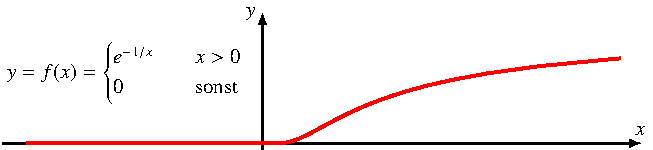
\includegraphics{chapters/020-variation/images/f.pdf}
\caption{Die beliebig oft stetig differenzierbare Funktion von
Satz~\ref{buch:variation:fundamentallemma:satz:glatt}
\label{buch:variation:fundamentallemma:fig:glatt}}
\end{figure}


\begin{satz}
\label{buch:variation:fundamentallemma:satz:glatt}
Die Funktion
\[
f(x)
=
\begin{cases}
e^{-1/x}&\qquad x>0\\
0&\qquad x\le 0
\end{cases}
\]
(siehe auch Abbildung~\ref{buch:variation:fundamentallemma:fig:glatt})
ist beliebig oft stetig differenzierbar.
\end{satz}

\begin{proof}
Es ist klar, dass die Funktion $f$ beliebig oft stetig differenzierbar
ist in jedem Punkt $x\ne 0$.
Es ist also nur nachzuweisen, dass $f(x)$ im Punkt $0$ beliebig
oft stetig differenzierbar ist.

Die ersten drei Ableitungen von $f(x)$ sind
\begin{align}
f'(x) &= \frac{1}{x^2} f(x)
\label{buch:variation:fundamentallemma:eqn:f1}
\\
f''(x) &= \frac{1-2x}{x^4}f(x)
\notag
\\
f'''(x) &= \frac{6x^2-6x+1}{x^6}f(x).
\notag
\end{align}
Daraus lässt sich die Vermutung ableiten, dass
\begin{equation}
f^{(n)}(x)
=
\frac{p_{n-1}(x)}{x^{2n}} f(x)
\label{buch:variation:fundamentallemma:eqn:fabl}
\end{equation}
ist, wobei $p_k(x)$ ein Polynom vom Grad $k$ ist.
Wir beweisen diese Vermutung mit Hilfe von vollständiger Induktion.
Die Induktionsverankerung für die $0$-te Ableitung ist trivial.

Wir nehmen jetzt im Sinne der Induktionsannahme an, dass die $n$-te
Ableitung die Form \eqref{buch:variation:fundamentallemma:eqn:fabl}
hat.
Wir müssen zeigen, dass dann auch $f^{(n+1)}(x)$ diese Form hat.
Dazu berechnen wir
\begin{align}
f^{(n+1)}(x)
&=
\frac{d}{dx}
\frac{p_n(x)}{x^{2n}} f(x)
\notag
\\
&=
\frac{p_n'(x)}{x^{2n}} f(x)
-2n
\frac{p_n(x)}{x^{2n+1}} f(x)
+
\frac{p_n(x)}{x^{2n}} f'(x).
\notag
\intertext{Mit der ersten Ableitung
\eqref{buch:variation:fundamentallemma:eqn:f1} wird dies zu}
&=
\frac{p_n'(x)}{x^{2n}} f(x)
-2n
\frac{p_n(x)}{x^{2n+1}} f(x)
+
\frac{p_n(x)}{x^{2n}} \frac{1}{x^2}f(x)
\notag
\\
&=
\frac{x^2p_n'(x) -2nxp_n(x)+p_n(x)}{x^{2n+2}} f(x).
\label{buch:variation:fundamentallemma:eqn:induktionsschritt}
\end{align}
Die Ableitung $p_n'(x)$ ist ein Polynom vom Grad $n-1$ und damit
ist $x^2p_n'(x)$ ein Polynom vom Grad $n+1$.
Ebenso ist $xp_n(x)$ ein Polynom vom Grad $n+1$ während
$p_n(x)$ ein Polynom vom Grad $n$ ist.
Der Zähler von
\eqref{buch:variation:fundamentallemma:eqn:induktionsschritt}
ist
\[
p_{n+1}(x)
=
x^2p_n'(x)+(1 -2nx)p_n(x),
\]
ein Polynom vom Grad $n+1$.
Damit ist der Induktionsschritt erfolgreich und die Behauptung betreffend
die Form von $f^{(n)}(x)$ ist bewiesen.

Es ist jetzt nur noch zu zeigen, dass der Grenzwert von $f^{(n)}(x)$
für $x\to 0+$ verschwindet.
Da das Polynom $p_n(x)$ stetig ist, folgt
\[
\lim_{x\to 0}
f^{(n)}(x)
=
\lim_{x\to 0}\frac{p_n(x)}{x^{2n}}f(x)
=
p_n(0) \lim_{t\to\infty} t^{2n} e^{-t}
=
0.
\]
Damit ist die beliebige stetige Differenzierbarkeit an der Stelle
$x=0$ gezeigt.
\end{proof}

Die Funktion $f(x)$ von 
Satz~\ref{buch:variation:fundamentallemma:satz:glatt} 
erfüllt noch nicht die Forderung, dass sie nur in einem vorgegebenen
Intervall von $0$ verschieden ist.

%
% g.tex -- template for standalon tikz images
%
% (c) 2021 Prof Dr Andreas Müller, OST Ostschweizer Fachhochschule
%
\documentclass[tikz]{standalone}
\usepackage{amsmath}
\usepackage{times}
\usepackage{txfonts}
\usepackage{pgfplots}
\usepackage{csvsimple}
\usetikzlibrary{arrows,intersections,math}
\begin{document}
\def\skala{3}
\def\a{-0.5}
\def\b{2.5}
\pgfmathparse{2/(\b-\a)}
\xdef\l{\pgfmathresult}
\begin{tikzpicture}[>=latex,thick,scale=\skala]

\draw[->] (-1,0) -- (3,0) coordinate[label={$x$}];
\draw[->] (0,-0.05) -- (0,1.1) coordinate[label={left:$y$}];

\begin{scope}
\clip (-1,-0.1) rectangle (2.9,1);
\draw[color=red,line width=1.2pt]
	plot[domain=0.25:10,samples=100] ({\a+1/\x},{exp(-\x)})
	-- (\a,0) -- (-1,0);
\draw[color=red,line width=1.2pt]
	plot[domain=0.25:10,samples=100] ({\b-1/\x},{exp(-\x)})
	-- (\b,0) -- (3,0);

\draw[color=blue,line width=1.2pt]
	plot[domain=\l:10,samples=100]
		({\a+1/\x},{exp(-\x)*exp(-1/(\b-\a-1/\x))}) -- (\a,0) -- (-1,0);
\draw[color=blue,line width=1.2pt]
	plot[domain=\l:10,samples=100]
		({\b-1/\x},{exp(-\x)*exp(-1/(-\a+\b-1/\x))}) -- (\b,0) -- (3,0);
\end{scope}

\draw (\a,-0.02) -- (\a,0.02);
\node at (\a,0) [below] {$a\mathstrut$};
\draw (\b,-0.02) -- (\b,0.02);
\node at (\b,0) [below] {$b\mathstrut$};
\node[color=blue] at ({0.5*(\a+\b)},0.12) {$g_{a,b}(x)$};
\node[color=red] at (\a,0.8) {$f(x-a)\mathstrut$};
\node[color=red] at (\b,0.8) {$f(b-x)\mathstrut$};

\end{tikzpicture}
\end{document}



\begin{satz}
\label{buch:variation:fundamentallemma:satz:gab}
Sei $f(x)$ die Funktion von
Satz~\ref{buch:variation:fundamentallemma:satz:glatt}.
Dann ist
\[
g_{a,b}(x)
=
f(x-a) f(b-x)
\]
eine unendlich oft stetig differenzierbare, nichtnegative Funktion mit Träger
$\supp g_{a,b}=(a,b)$.
\end{satz}

Die Funktionen $g_{a,b}(x)$ sind beliebig oft differenzierbar und nur im
Intervall $[a,b]$ von $0$ verschieden und sogar positiv.
Weil sie stetig sind, sind sie auch integrierbar, man kann also das
Integral über $\mathbb{R}$ berechnen und die Funktion damit normieren.
Die neue Funktion
\[
\frac{1}{N}
\tilde{g}_{a,b}(x)
\qquad\text{mit}\;
N
=
\int_{-\infty}^{\infty}g_{a,b}(x)\,dx
=
\int_a^b g_{a,b}(x)\,dx
\]
ist immer noch beliebig oft stetig differenzierbar und hat zusätzlich die
Eigenschaft
\[
\int_{-\infty}^{\infty}
\tilde{g}_{a,b}(x)\,dx
=
\int_a^b
\tilde{g}_{a,b}(x)\,dx
=
1.
\]
Wir formulieren dieses Resultat als Satz.

\begin{satz}
\label{buch:variation:satz:gabeins}
Zu jedem Intervall $[a,b]$ gibt es eine beliebig oft stetig
differenzierbare Funktion $g(x)$, genau das Intervall $[a,b]$
als Träger hat und deren Integral über $[a,b]$ den Wert $1$ hat.
\end{satz}

%
% Das Fundamentallemma
%
\subsection{Das Fundamentallemma}
Mit der Funktion $g_{a,b}(x)$ von
Satz~\ref{buch:variation:fundamentallemma:satz:gab}
lässt sich jetzt das Fundamentallemma in der folgenden Form
leicht beweisen.

\begin{satz}[Fundamentallemma]
\label{buch:variation:fundamentallemma:satz:fundamentallemma}
Wenn für die stetige Funktion $f\colon[a,b]\to\mathbb{R}$ 
\begin{equation}
\int_a^b f(x)\varphi(x)\,dx = 0
\label{buch:variation:fundamentallemma:eqn:fundamentalbed}
\end{equation}
gilt für jede beliebig oft stetig differenzierbare Funktion $\varphi(x)$ 
dann ist $f(x)=0$.
Das Resultat gilt selbst dann, wenn
\eqref{buch:variation:fundamentallemma:eqn:fundamentalbed}
nur für beliebig oft stetig differenzierbare Funktionen $\varphi(x)$ 
gilt, die ausserdem an den Intervallenden verschwinden:
$\varphi(a)=\varphi(b)=0$.
\end{satz}

\begin{proof}
Wir zeigen mit Hilfe eines Widerspruchs, dass es keinen Punkt $x_0\in[a,b]$
geben kann, für den $f(x_0)\ne 0$ ist.
Dazu nehmen wir also an, dass $f(x_0)\ne 0$ ist.
Falls $f(x_0)<0$ ist, ersetzen wir $f$ durch $-f$, 
die Bedingung
\eqref{buch:variation:fundamentallemma:eqn:fundamentalbed}
ändert sich dadurch nicht.
%
% fundamentallemma.tex -- Fundamentallemma
%
% (c) 2021 Prof Dr Andreas Müller, OST Ostschweizer Fachhochschule
%
\documentclass[tikz]{standalone}
\usepackage{amsmath}
\usepackage{times}
\usepackage{txfonts}
\usepackage{pgfplots}
\usepackage{csvsimple}
\usetikzlibrary{arrows,intersections,math}
\definecolor{darkgreen}{rgb}{0.0,0.6,0.0}
\definecolor{darkred}{rgb}{0.8,0.0,0.0}
\begin{document}
\def\skala{1}
\def\X{4.555}
\def\X{4.7}
\def\e{0.85}
\begin{tikzpicture}[>=latex,thick,scale=\skala,
declare function={
	f(\t) = (-0.4*\t)+4-1.5*sin(50*\t)-1.5*cos(120*\t);
}]

\fill[color=darkred!20]
	plot[domain=-180:180] ({\X+\e*\x/180},{cos(\x)+1})
	--
	cycle;

\draw[color=blue!20,line width=1.2pt]
	plot[domain=0.2:7.8,samples=100] ({\x},{f(\x)});
\begin{scope}
\clip ({\X-\e},0) rectangle ({\X+\e},5.4);
\draw[color=blue,line width=1.4pt]
	plot[domain={\X-2*\e}:{\X+2*\e},samples=100] ({\x},{f(\x)});
\end{scope}
\node[color=blue] at ({\X-0.8*\e},{f(\X-0.8*\e)}) [left] {$f(x)$};
%\node[color=blue] at ({\X},{f(\X)}) [above] {$f(x_0)$};
\draw[color=blue,line width=0.4pt] (0,{f(\X)}) -- ({\X},{f(\X)});
\draw[color=blue] (-0.05,{f(\X)}) -- (0.05,{f(\X)});
\node[color=blue] at (-0.05,{f(\X)}) [left] {$f(x_0)$};

\draw[color=blue,line width=0.4pt] ({\X},0) -- ({\X},{f(\X)});
\node at (\X,-0.05) [below] {$x_0\mathstrut$};

\draw[color=darkgreen,line width=0.4pt] ({\X-\e},0) -- ({\X-\e},5.2);
\draw[color=darkgreen,line width=0.4pt] ({\X+\e},0) -- ({\X+\e},5.2);
\draw[color=darkgreen,line width=0.4pt] (0,{0.5*f(\X)}) -- ({\X},{0.5*f(\X)});
\draw[color=darkgreen] (-0.05,{0.5*f(\X)}) -- (0.05,{0.5*f(\X)});
\node[color=darkgreen] at (-0.05,{0.5*f(\X)})
	[left] {$\frac12f(x_0)\mathstrut$};
\draw[color=darkgreen,line width=1.2pt]
	({\X+\e},{0.5*f(\X)}) 
	-- 
	({\X-\e},{0.5*f(\X)});
%\node[color=darkgreen] at ({\X},{0.5*f(\X)}) [above] {$\frac12f(x_0)$};
\draw[color=darkgreen] ({\X-\e},-0.05) -- ({\X-\e},0.05);
\node[color=darkgreen] at ({\X-\e},-0.05) [below left] {$x_0-\delta\mathstrut$};
\draw[color=darkgreen] ({\X+\e},-0.05) -- ({\X+\e},0.05);
\node[color=darkgreen] at ({\X+\e},-0.05) [below right] {$x_0+\delta\mathstrut$};

\fill[color=blue] ({\X},{f(\X)}) circle[radius=0.08];

\draw[->] (-0.1,0) -- (8.5,0) coordinate[label={$x$}];
\draw[->] (0,-0.1) -- (0,5.4) coordinate[label={left:$y$}];

\draw[color=darkred,line width=1.2pt]
	(0.5,0)
	--
	({\X-\e},0)
	--
	plot[domain=-180:180] ({\X+\e*\x/180},{cos(\x)+1})
	--
	({\X+\e},0)
	--
	(7.5,0);
\node[color=darkred] at ({\X+0.5*\e},1) [right] {$g(x)$};

\draw[line width=0.4pt] (0.5,0) -- (0.5,5.2);
\draw (0.5,-0.05) -- (0.5,0.05);
\node at (0.5,-0.05) [below] {$x_1\mathstrut$};

\draw[line width=0.4pt] (7.5,0) -- (7.5,5.2);
\draw (7.5,-0.05) -- (7.5,0.05);
\node at (7.5,-0.05) [below] {$x_2\mathstrut$};

\end{tikzpicture}
\end{document}


Wir dürfen daher annehmen, dass $f(x_0)>0$ ist
(Abbildung~\ref{buch:variation:fundamentallemma:fig:beweis}).
Da $f$ stetig ist, gibt es ein Intervall $[x_0-\varepsilon,x_0+\varepsilon]$
derart, dass $f(x)> \frac12 f(x_0)$ für
$x\in[x_0-\varepsilon,x_0+\varepsilon]$ gilt.
Dann gilt für das Integral
\[
\int_a^b
f(x)
g_{x_0-\varepsilon,x_0+\varepsilon} (x)
\,dx
>
\frac{f(x_0)}{2}
\int_a^b
g_{x_0-\varepsilon,x_0+\varepsilon} (x)
\,dx
>
0
\]
im Widerspruch zur Bedingung
\eqref{buch:variation:fundamentallemma:eqn:fundamentalbed}.
Der Widerspruch zeigt, dass $f(x)=0$ sein muss.
\end{proof}

%
% Skalarproduktformulierung des Fundamentallemmas
%
\subsection{Skalaproduktformulierung des Fundamentallemmas}
Die Richtungsableitung einer Funktion endlich vieler Variablen 
konnte als Skalarprodukt mit dem Gradienten geschrieben werden und
das Fundamentallemma hat besagt, dass der Gradient verschwindet,
wenn alle Richtungsableitungen verschwinden.
Diese Schlussweise ist auch für Funktionen möglich, wenn man Funktionen
ein Skalarprodukt definieren kann.

\begin{definition}[$L^2$-Skalarprodukt]
Das {\em Skalarprodukt} zweier quadratintegrierbarer Funktion $f$ und $g$
auf dem Intervall $[a,b]$ ist definiert durch
\[
\langle f,g\rangle
=
\int_a^b f(x)g(x)\,dx.
\]
\end{definition}

\begin{satz}[Fundamentallemma, Skalarproduktform]
Wenn für eine stetige Funktion $f\colon[a,b]\to\mathbb{R}$ das Skalarprodukt
\[
\langle f,\varphi\rangle = 0
\]
ist für jede unendlich oft differenzierbare Funktion $\varphi$ auf dem
Intervall $[a,b]$, dann ist $f=0$.
\end{satz}


